\chapter{Daten}

Wie bei jeder Anwendung von maschinellen Lernverfahren sind die zugrundeliegenden Daten von äußerster Wichtigkeit.
Im Rahmen dieser Masterarbeit wurden zu Beginn existierende Aufnahmen und Track benutzt, 
bevor dann selbst am Schüttgutsortierer des Fraunhofer IOSBs Aufnahmen gemacht wurden.


\section{Eigene Aufnahmen}

\subsection{Kamera}

[Beschreibung von der Bonito Kamera, stats usw.]
Zur Aufnahme der Trainingsdaten wurde eine Bonito CL-400 200 FPS Kamera benutzt,
die oberhalb des Förderbandes angebracht wird.

\begin{figure}
    \centering
    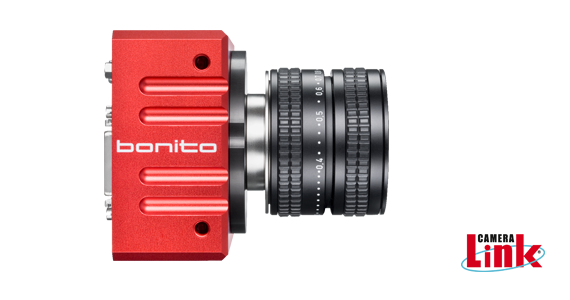
\includegraphics[width=\textwidth]{img/banner-Bonito_cropped}
    \caption{Zur Aufname verwendete Kamera [TODO: Quelle Bild]}
    \label{piechartSchuettgut}
\end{figure}

\subsection{Schüttgüter}

Aufgenommen wurden vier verschiedene Schüttgüter:

\begin{itemize}
    \item Kugeln
    \item grüne Pfefferkörner
    \item Zylinder
    \item Weizenkörner
\end{itemize}

Die Kugeln und der Pfeffer sowie die Zylinder und die Weizenkörner bilden jeweils 
ein Paar aus einem geometrischen Körper und einem echten Objekt, das grob dessen Form ähnelt.
[Details]

\subsection{Pipeline}

Die Bilder wurden in Batches von je 3500 gesammelt.
Die Bonito Kamera schreibt sie als eine Bayer-Matrix in Bitmap Dateien.
Auf Grund der Menge an Bildern war es sinnvoll die Dateien in das png Format zu übertragen.
Die Features, die für das Trainieren der Netze benutzt werden, sind die Koordinaten der Mittelpunkte der Objekte.
Um diese zu bestimmten müssen zunächst die Dateien mittels \textit{Demosaicing} rekonstruiert werden um gewöhnliche RGB Bilder zu erhalten.
[Reference Debayer script?]
Auf diesen kann dann eine Segmentierung vorgenommen werden.
Hierzu wurde die Computer Vision Library OpenCV benutzt.
Das Ergebnis des Segmentierungsscripts [Reference segement.py] ist ein CSV File für jedes Batch.
Eine Zeile repräsentiert ein Bild aus dem Batch, also einen Zeitschritt.
Zu Beginn jeder Zeile steht zunächst die Frame Nummer, gefolgt von der Anzahl der detektierten Partikel. 
Die X- und Y-Koordinaten von der detektierten Partikeln sind dann links angehängt

\begin{table}[ht]
\begin{adjustbox}{width=1\textwidth}
\begin{tabular}{c|c|c|c|c|c}%
    %\bfseries Person & \bfseries Matr.~No.% specify table head
    
    \bfseries TrackID\_1\_X & \bfseries TrackID\_1\_Y & \bfseries TrackID\_2\_X  & \bfseries TrackID\_2\_Y & \bfseries TrackID\_3\_X & \bfseries TrackID\_3\_Y
    \csvreader[head to column names]{docExample.csv}{}% use head of csv as column names
    {\\\hline\csvcoli&\csvcolii&\csvcoliii&\csvcoliv&\csvcolv&\csvcolvi} % specify your coloumns here
    \end{tabular}
\end{adjustbox}
\caption{Beispielhafter Ausschnitt aus einem CSV File} 
\end{table} 

\subsection{Menge}

Insgesamt wurden 177954 Bilder aufgenommen.

Es wurden 
7002 Kugeln in 14 Batches,
7056 Pfefferkörner in 13 Batches,
17049 Zylinder in 11 Batches
und 8549 Weizenkörner in 13 Batches aufgenommen.

\begin{figure}
    \centering
    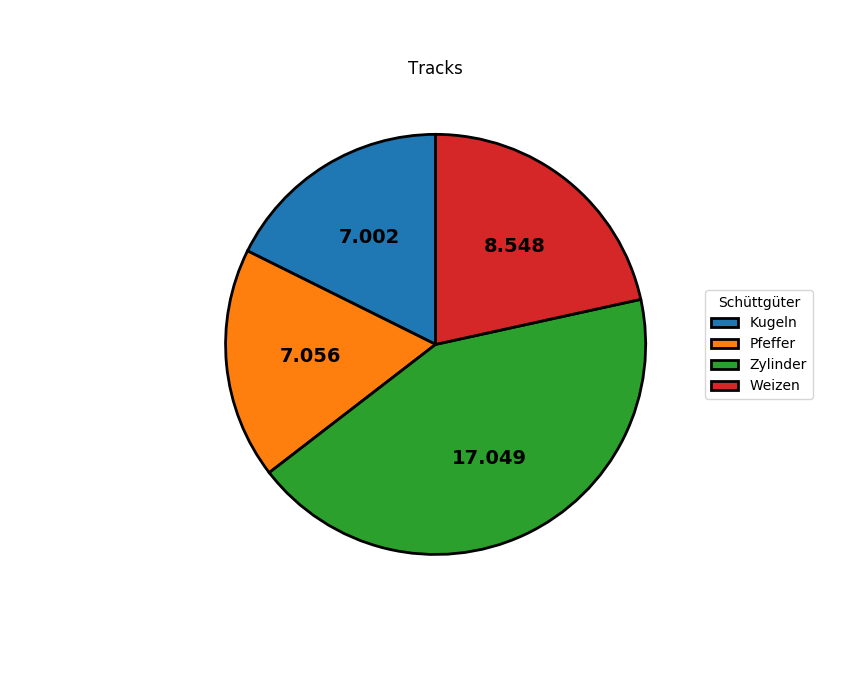
\includegraphics[width=\textwidth]{img/scaledPieChart-trimmed}
    \caption{Verteilung Schüttgut Elemente nach Sorte}
    \label{piechartSchuettgut}
\end{figure}

Bei einer FeatureSize von 5 ergeben sich bei den Kugeln so 98.966 Feature-Label Paare.
Die Pfefferkörner haben dann 105.101 Feature-Label Paare,
bei den Zylindern kommt man auf 244.422 Feature-Label Paare
und bei den Weizenkörner 132.140 Feature-Label Paare.

